\documentclass[tikz,14pt,border=10pt,subpreambles=true]{standalone}
\usepackage{pgfplots}
\usepackage{pgfplotstable}
\pgfplotsset{compat = newest}
\begin{document}
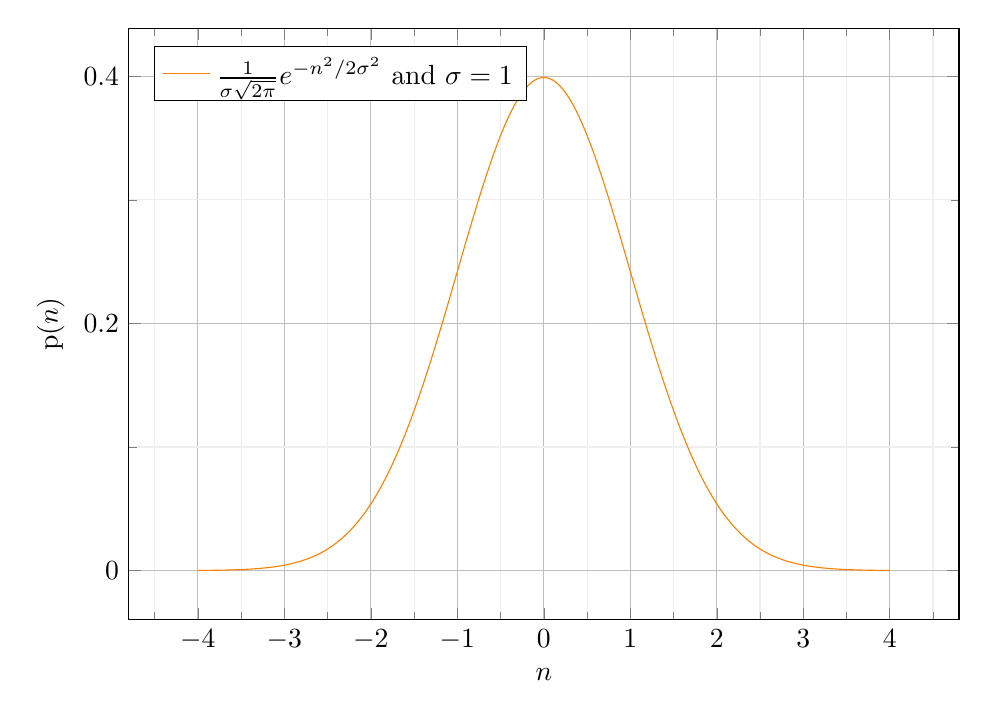
\begin{tikzpicture}
\begin{axis}[
    width = \textwidth,
    height = 0.75\textwidth,
    xtick distance = 1,
    ytick distance = 0.2,
    grid = both,
    minor tick num = 1,
    major grid style = {lightgray},
    minor grid style = {lightgray!25},
    xlabel = {$n$},
    ylabel = {p($n$)},
    legend cell align = {left},
    legend pos = north west
]
% plot data line code
\addplot [
    domain=-4.0:4.0, 
    samples=200, 
    color=orange,
    ]
    {(1/(1*sqrt(2*pi))*e^((-x^2)/(2*1^2))};
\addlegendentry{$\frac{1}{\sigma \sqrt{2 \pi}} e^{-n^2 / 2 \sigma^2}$ and $\sigma=1$}
\end{axis}
 
\end{tikzpicture}
\end{document}